\chapter{Data-Driven Control}~\label{ch:DDC}
Data-driven control is an emerging paradigm in control theory that focuses on designing controllers directly from data, without relying on explicit parametric models of the system dynamics. This chapter explores the principles and methodologies of predictive control, both in the context of known system models and in scenarios where only data is available. We focus specifically on finite-time linear quadratic tracking problems, and highlight the advantages of the behavioral framework in enabling data-driven control strategies.

\section{Linear Quadratic Tracking}
Finite-time linear quadratic tracking (LQT) is a fundamental optimal control problem~\cite{anderson2007} where the objective is to minimize a quadratic cost function over a finite time horizon while tracking a desired reference trajectory. Consider a discrete-time \Nref*{def:lti} given by 
\begin{equation}
    \begin{cases}
        x(t+1) = A x(t) + B u(t), \\
        y(t) = C x(t) + D u(t),
    \end{cases}
\end{equation}
where $A \in \R^{n \times n}, B \in \R^{n \times m}, C \in \R^{p \times n}, D \in \R^{p \times m}$ are system matrices, $x(t) \in \R^n$ is the state vector, $u(t) \in \R^m$ is the control input, and $y(t) \in \R^p$ is the output vector. Given a desired trajectory $r = (r_0, r_1, \cdots) \in (\R^p)^\N$, input constraint set $\mathcal{U} \subseteq \R^m$, and output constraint set $\mathcal{Y} \subseteq \R^p$, we wish to apply control inputs such that the output tracks the reference trajectory while satisfying the constraints and optimizing a cost function.

In the case where the system is \emph{known}, i.e., the matrices $A, B, C, D$ are given, the finite-horizon LQT problem is approached using \emph{Model Predictive Control}.

\subsection{Model Predictive Control}\label{sec:mpc}
Model Predictive Control (MPC) is an advanced control strategy that utilizes an explicit model of the system to predict future behavior and optimize control actions over a finite horizon~[\cite{camacho2007},~\cite{ferramosca2009}]. Consider the optimization problem:
\begin{equation}\label{eq:mpc}
    \begin{aligned}
        & \underset{u,x,y}{\text{minimize}} && \sum_{k=0}^{N-1} \left( \lVert y_k - r_{t+k} \rVert_Q^2 + \lVert u_k \rVert_R^2 \right) \\
        & \text{subject to} && x_{k+1} = A x_k + B u_k, \\
        & && y_k = C x_k + D u_k, \\
        & && x_0 = \hat{x}(t), \\
        & && u_k \in \mathcal{U}, \forall k \in \{0, \ldots, N-1\} \\
        & && y_k \in \mathcal{Y}, \forall k \in \{0, \ldots, N-1\},
    \end{aligned}
\end{equation}
where $N \in \Z_{> 0}$ is the time horizon, $u = (u_0, u_1, \ldots, u_{N-1}), x = (x_0, x_1, \ldots, x_N)$, $y = (y_0, y_1, \ldots, y_{N-1})$ are the decision variables, and $r_{t+k}$ is the desired reference at time $t+k$, where $t \in \Z_{>0}$ is the time at which the optimization is solved. The matrices $Q \succeq 0$ and $R \succ 0$ are weighting matrices for the output tracking error and control effort, respectively. The initial state $\hat{x}(t)$ is typically obtained from state estimation or measurement at time $t$.

The classical MPC algorithm operates in a \emph{receding horizon} fashion. The algorithm is summarized in Algorithm~\ref{alg:mpc} and illustrated in Figure~\ref{fig:mpc_schematic}.

\begin{algorithm}[H]
\SetKwInOut{Input}{Input}
        \Input{$(A,B,C,D)$, reference trajectory $r$, past input/output data $(u,y)$, constraint sets $\mathcal{U}, \mathcal{Y}$, weighting matrices $Q,R$, time horizon $N$}
    \BlankLine
        Generate state estimate $\hat{x}(t)$ from past data $(u,y)$.\;
        Solve~\eqref{eq:mpc} for $u^* = (u_0^*, u_1^*, \ldots, u_{N-1}^*)$.\;
        Apply inputs $(u(t), \ldots, u(t+s)) = (u^*_0, \ldots, u^*_s)$ for some $s \leq N-1$.\;
  	    Set $t$ to $t+s$ and update past input/output data.\;
        Return to start.
    \caption{Model Predictive Control}
    \label{alg:mpc}
\end{algorithm}

\begin{figure}[h!]
    \centering
    \begin{tikzpicture}[
    scale=1.5,
    >=Stealth,
    timeline/.style={thick, ->},
    horizon/.style={decorate, decoration={brace, amplitude=5pt}},
    trajectory/.style={},
    ref trajectory/.style={trajectory, black, ultra thick, dotted, dash pattern=on 2pt off 10pt},
    actual trajectory/.style={trajectory, red, ultra thick, dotted, dash pattern=on 2pt off 10pt},
    control trajectory/.style={trajectory, blue, thin},
    futcontrol trajectory/.style={trajectory, blue, thin, dashed},
    time label/.style={font=\small}
    ]

    \def\Tini{3}   % Past horizon
    \def\N{5}      % Future horizon
    \def\L{8}      % Total horizon = Tini + N
    \def\usteps{%
    (0,0.50) -- (0.5,0.50)
    -- (0.5,0.5) -- (1.0,0.5)
    -- (1.0,0.35) -- (1.5,0.35)
    -- (1.5,0.75) -- (2.0,0.75)
    -- (2.0,0.45) -- (2.5,0.45)
    -- (2.5,0.65) -- (3.0,0.65)
    }
    \def\futsteps{
    (3.0, 0.65) -- (3.0,0.50) -- (3.5,0.50)
    -- (3.5,0.50) -- (4.0,0.50)
    -- (4.0,0.50) -- (4.5,0.50)
    -- (4.5,1.2) -- (5.0,1.2)
    -- (5.0,0.58) -- (5.5,0.58)
    -- (5.5,0.75) -- (6.0,0.75)
    -- (6.0,0.35) -- (6.5,0.35)
    -- (6.5,0.47) -- (7.0,0.47)
    -- (7.0,0.47) -- (7.5,0.47)
    -- (7.5,0.47) -- (8.0,0.47)
    }

    \draw[gray!80, timeline] (-0.5, 0) -- (\L+0.5, 0);


    \draw[gray!80, thin] (3, 0.2) -- (3, -0.2) node[below, time label] {$k$};
    \draw[gray!80, thin] (8, 0.2) -- (8, -0.2) node[below, time label] {$N$};


    \draw[->, gray!80, thick] (\Tini, -0.1) -- (\Tini, 4);

    \draw[ref trajectory] (0, 2) to[out=0, in=170] (\L, 2.7) node[above left, yshift=2mm] {reference $\mathbf{r}$};
    \draw[trajectory] (0, 2) to[out=0, in=170] (\L, 2.7);


    \draw[actual trajectory] (0, 1) to[out=10, in=170] 
        (\L, 2.5) node[below left] {output $\mathbf{y}$};
    \draw[trajectory, red] (0,1) to [out=8, in=19] (\Tini, 1.84);
    \draw[thin, densely dashed, red] (0,1) to[out=10,in=170] (\L, 2.5);

    \draw[control trajectory] \usteps;
    \draw[futcontrol trajectory] \futsteps node[above left, yshift=5mm] {control action $\mathbf{u}$};


    \node at (\Tini/1.5, 3.9) {\textcolor{gray}{past}};
    \draw[<-, gray!80] (\Tini/1.5-0.7, 3.6) to (\Tini/1.5+0.7, 3.6);
    \node at (\Tini + \N/5, 3.9) {\textcolor{gray}{future}};
    \draw[->, gray!80] (\Tini+\N/5-0.7, 3.6) to (\Tini+\N/5+0.7, 3.6);

    \draw[<->, gray!80] (\Tini, -0.8) to (8,-0.8) node[below left] {\textcolor{gray}{prediction horizon}};

    \end{tikzpicture}
    \caption{Classical MPC in a receding horizon fashion. At each time step, an optimization problem is solved over a future horizon using the current state estimate and past data. The first $s$ control inputs are applied, and the horizon recedes forward in time.}~\label{fig:mpc_schematic}
\end{figure}

\newpage
\subsection{Data-Driven Predictive Control}

When the system model is \emph{unknown}, i.e., the matrices $A, B, C, D$ are not available, traditional model-based control strategies like MPC cannot be directly applied. Instead, we turn to data-driven predictive control methods [e.g. DeePC~\cite{jeremy2019}] that leverage historical input-output data to design controllers without explicit knowledge of the system dynamics. The behavioral framework introduced in Chapter~\ref{ch:Behaviors} provides a powerful toolset for such data-driven approaches, since it bypasses the need for parametric models and directly utilizes data to characterize system behavior.

On a finite-horizon, the problem can be formulated as follows. Given,
\begin{itemize}
    \item an LTI system $\Sigma = (\T, \W, \Be)$, with $\W = \R^q$, and $\T = [1,N]$,
    \item an initial trajectory $w_{\textrm{ini}} \in \Be |_{\T_{\textrm{past}}}$ with $\T_{\textrm{past}} = [1, T_{\textrm{ini}}]$,
    \item a reference trajectory $w_{\textrm{ref}} \in {(\R^q)}^{\T_{\textrm{fut}}}$, with $\T_{\textrm{fut}} = [T_{\textrm{ini}}+1, N]$,
    \item a symmetric positive semi-definite weighting matrix $\Phi \in \R^{q \times q}$,
\end{itemize}
the linear quadratic tracking problem is to find a trajectory $w_{\textrm{fut}} \in \Be |_{\T_{\textrm{fut}}}$ that solves the optimization problem
\begin{equation}\label{eq:lqt_behavioral}
    \begin{aligned}
        \underset{w_{\textrm{fut}} \in {(\R^q)}^{\T_{\textrm{fut}}}}{\text{minimize}} && \sum_{k=T_{\textrm{ini}}+1}^{N} \lVert w_{\textrm{fut}}(k) - w_{\textrm{ref}}(k) \rVert_{I \otimes \Phi}^2 \\
       && \text{subject to} \quad w = \begin{bmatrix} w_{\textrm{ini}} \\ w_{\textrm{fut}} \end{bmatrix} \in \Be.
    \end{aligned}
\end{equation}

\begin{Note}
    The reference trajectory $w_{\textrm{ref}}$ need not be in the behavior $\Be$. For instance, step inputs with sudden changes can be used as reference trajectories, even if they are not achievable by the system.
\end{Note}

If a parametric model of the system behavior is available---for example a state-space representation---then the optimization problem~\eqref{eq:lqt_behavioral} is equivalent~\cite{jeremy2019} to the classical MPC problem~\eqref{eq:mpc} described in Section~\ref{sec:mpc}. However, in the absence of such a model, we can utilize the behavioral framework to reformulate the problem in a data-driven manner.

\section{Robust Least-Squares for Data-Driven Control}
Predictive control methods like DeePC~\cite{jeremy2019} rely on the availability of persistently exciting input-output data to construct Hankel matrices that capture the system's behavior. However, in practical scenarios, the collected data may be corrupted by noise, outliers, or other uncertainties, which can adversely affect the performance of data-driven controllers. To address these challenges, robust least-squares techniques can be employed to enhance the resilience of data-driven predictive control methods against data imperfections.

\subsection{Geometric Approach to Robust Least-Squares}
We consider a geometric approach to robust least-squares problem in the context of linear quadratic tracking. Building up from~\eqref{eq:lqt_behavioral}, we formulate:
\begin{equation}\label{eq:robust_lqt}
    \begin{split}
    \min_{w \in \R^n} & \max_{\Sy \in \B_{\rho}(\hat{\Sy})} \lVert w - w_{\textrm{ref}} \rVert^2 \\
    \text{subject to} & \quad \begin{cases} w \in \Sy,\\
          w|_{\T_{\textrm{past}}} = w_{\textrm{ini}} \end{cases}
    \end{split}
\end{equation}
Here, 
\begin{itemize}
    \item $\B_{\rho}(\hat{\Sy}) \subseteq \Gr(k,n)$ is a ball of radius $\rho$ centered at $\hat{\Sy} \equiv \Be|_{[1,L]}$ which is obtained via behavioral system identification.
    \item $n = qL, k = m(\Be)L+n(\Be)$ where $m(\Be), n(\Be)$ are the output and state dimensions of the behavior $\Be$ respectively.
    \item $w_{\textrm{ref}} = \textrm{col}(w_{\textrm{ini}}, w_{\textrm{ref,f}}) \in {(\R^q)}^\T$ is the reference trajectory over the horizon $N$.
    \item $w_{\textrm{ini}} \in {(\R^q)}^{\T_{\textrm{past}}}$ is the initial trajectory over the horizon $N$.
\end{itemize}

\subsection{Constraints}
The constraints in~\eqref{eq:robust_lqt} are briefly discussed here.

\begin{table}[h]
    \centering
    \begin{tabular}{p{0.46\linewidth}|p{0.46\linewidth}}
        % \hline
        % anchor labels so references like \eqref{const1}/\eqref{const2} work
        % \refstepcounter{equation}\label{const1} (\theequation) & \refstepcounter{equation}\label{const2} (\theequation) \\
        To enforce the constraint $w \in \Sy$, we utilize the orthogonal projection onto the subspace $\Sy$. Specifically, we take the transformation
        \begin{equation}
            w = P_{\Sy} x = YY^\top x,
        \end{equation}
        where $P_{\Sy}$ is the orthogonal projection matrix onto the subspace $\Sy$, and $Y \in \R^{n \times k}$ is an orthonormal basis for $\Sy$. The variable $x \in \R^n$ is a new decision variable that allows us to express $w$ in terms of the subspace $\Sy$. & The past constraint $w|_{\T_{\textrm{past}}} = w_{\textrm{ini}}$ is a linear equality constraint that can be expressed in matrix form as
        \begin{equation}
            M w = w_{\textrm{ini}},
        \end{equation}
        where $M = [\I_{q T_{\textrm{ini}}} \quad 0] \in \R^{q T_{\textrm{ini}} \times n}$ is a selection matrix that extracts the components of $w$ corresponding to the past horizon $\T_{\textrm{past}}$.
        Substituting the expression for $w$ into this constraint gives
        \begin{equation}
            M YY^\top x = w_{\textrm{ini}}.
        \end{equation} 
        % \hline
    \end{tabular}
    \caption{Reformulation of constraints in~\eqref{eq:robust_lqt}.}~\label{tab:constraints_reformulation}
\end{table}

\subsection{Reformulated Problem}
Substituting the expressions for $w$ and the constraints into the robust least-squares problem~\eqref{eq:robust_lqt}, we obtain the reformulated optimization problem:
\begin{equation}\label{eq:reformulated_robust_lqt}
    \begin{split}
    \min_{x \in \R^n} & \max_{\Sy \in \B_{\rho}(\hat{\Sy})} \lVert YY^\top x - b \rVert^2 \\
    \text{subject to} & \quad M YY^\top x = z,
    \end{split}
\end{equation}
where $b = w_{\textrm{ref}}$ and $z = w_{\textrm{ini}}$ for notational convenience. This problem is exactly in the form of the constrained robust least-squares problem discussed in Chapter~\ref{ch:Preliminaries}, Subsection~\ref{subsec:cons-robust-ls}, and can be solved using the geometric approach outlined therein.

\begin{Note}
    The cost function in~\eqref{eq:reformulated_robust_lqt} can be modified to include weighting matrices or regularization terms as needed (see Subsection~\ref{subsec:reg}). For instance, if we wish to penalize deviations in certain components of the trajectory more heavily, we can introduce a weighting matrix $\Phi$ into the cost function.
\end{Note}

Thus, the algorithm for data-driven predictive control using (regularized) robust least-squares can be summarized as follows:

\begin{algorithm}[H]
\SetKwInOut{Input}{Input}\SetKwInOut{Output}{Output}
        \KwData{Subspace estimate $\hat{\Sy} \in \Gr(k,n)$, System simulator $(A,B,C,D)$}
        \Input{Initial trajectory $z = w_{\textrm{ini}} \in {(\R^q)}^{\T_{\textrm{ini}}}$, Reference trajectory $r \in {(\R^p)}^{\T}$}
        \Output{Optimal trajectories $w^* \in {(\R^q)}^{\T}$}
    \BlankLine\While{$t \in [1,T]$} {
        Update $z = w_{\textrm{ini}} = [u_{\textrm{past}}^\top, y_{\textrm{past}}^\top]^\top$ from past data.\;
        Update $w_{\textrm{ref,f}} = [0^\top, r^\top]^\top$ from reference data.\;
        Define $b = [z^\top, w_{\textrm{ref,f}}^\top]^\top$.\;
        Solve Algorithm~\ref{alg:cons-robust-ls} with inputs $(\hat{\Sy}, b, z)$ to obtain $(x^*,Y^*)$.\;
        Obtain optimal trajectory $w^* = Y^* {Y^*}^\top x^*$.\;
        Apply control inputs $u^*(t), \ldots, u^*(t+s)$ for some $s \leq N-1$.\;
        Set $t$ to $t+s$ and update past input/output data.\;
    }
    \caption{Data-Driven Predictive Control via Robust Least-Squares}
\end{algorithm}

\section{Results}
The proposed data-driven predictive control algorithm using robust least-squares has been evaluated on various LTI systems. The results demonstrate improved tracking performance and robustness against data imperfections compared to traditional least-squares approaches. 

\subsection{Double Integrator System}
Consider a simple double-integrator system $\ddot{x}(t) = \dfrac{F(t)}{m}$, given in discrete time as
\begin{equation}
\begin{split}
    \begin{bmatrix}
        x_{k+1} \\ v_{k+1}
    \end{bmatrix} &= \begin{bmatrix}
        1 & h \\ 0 &  1
    \end{bmatrix} \begin{bmatrix}
        x_k \\ v_k
    \end{bmatrix} + \begin{bmatrix}
        \frac{h^2}{2m} \\ \frac{h}{m}
    \end{bmatrix}u_k  \\
    y_k &= \begin{bmatrix}
        1 & 0
    \end{bmatrix} \begin{bmatrix}
        x_k \\ v_k
    \end{bmatrix} + \eta_k
\end{split}
\end{equation}
where $x_k = x(t_k), v_k = \dot{x}(t_k)$ are the states, $h = t_{k+1} - t_k$ is the simulation time-step, and $\eta_k \sim \mathcal{N}(0, \sigma^2)$ is measurement noise. The system parameters are set to $m = 1$ kg, $h = 0.5$ s. The control objective is to track a reference trajectory $r = 1$ m over a horizon of $N$ time steps, with a random initial condition $[x_0, v_0]$.

\subsubsection{Offline System Identification}
To identify the behavior $\Be$ of the double-integrator system, we collect input-output data by simulating the system with random control inputs $u_k$ drawn from a uniform distribution over $[-1, 1]$ N. The output measurements $y_k$ are corrupted with Gaussian noise. A total of $T = 115$ time steps of data is collected, and a persistently exciting input sequence of order $L = T_{\textrm{ini}}+N = 35$ is ensured. Using this data, we construct the Hankel matrix and extract the subspace estimate $\hat{\Sy}$ using the methods outlined in Chapter~\ref{ch:Behaviors}. Thus, we summarize the following parameters from system identification of the double-integrator system in Table~\ref{tab:sysid_params_double_integrator}.
\begin{table}[h]
    \centering
    \begin{tabular}{l|c}
        \textbf{Parameter} & \textbf{Value} \\
        \hline 
        \hline
        Number of inputs $m(\Be)$ & 1 \\
        Number of outputs $p(\Be)$ & 1 \\
        Number of states $n(\Be)$ & 2 \\
        Dimension of behavior $k$ & 37 \\
        Data length $T_d$ & 115 \\
        Future horizon $N$ & 25 \\
        Past horizon $T_{\textrm{ini}}$ & 10 \\
        Total horizon $L$ & 35 \\
        Subspace dimension $\dim(\hat{Y})$ & 70 $\times$ 37 \\
        \hline
    \end{tabular}
    \caption{System identification parameters for double-integrator system.}~\label{tab:sysid_params_double_integrator}
\end{table}

\subsubsection{Online Predictive Control}
With the identified subspace $\hat{\Sy}$, we implement the data-driven predictive control algorithm using robust least-squares. The control inputs are computed over a receding horizon of $T = 50$ time steps, with the first $s = 1$ control input applied at each iteration. The reference trajectory is set to $r_k = 1$ m for all $k$. The robust least-squares problem is solved using the geometric approach outlined in Chapter~\ref{ch:Preliminaries}, with a ball radius $\rho$ chosen based on the noise level in the data.

Figures~\ref{fig:ddpc_noiseless} and~\ref{fig:conv_noiseless} illustrate the system simulations and optimization convergence for the case of no measurement noise ($\sigma = 0$). The results demonstrate effective tracking of the reference trajectory and convergence of the optimization process. The parameters/results for the simulations are summarized in Table~\ref{tab:ddpc_params_double_integrator}.
\begin{table}[h]
    \centering
    \begin{tabular}{l|c}
        \textbf{Parameter} & \textbf{Value} \\
        \hline 
        \hline
        $\rho$ & 0.1$^\circ$ \\
        $\gamma$ & 5.0 \\
        Total Run-Time & 4.27 s \\
        Tracking Time & 15 s \\
        \hline
    \end{tabular}
    \caption{Simulation parameters/results for $\sigma=0$ (no noise)}
    \label{tab:ddpc_params_double_integrator}
\end{table}
\begin{figure}[h]
    \centering
    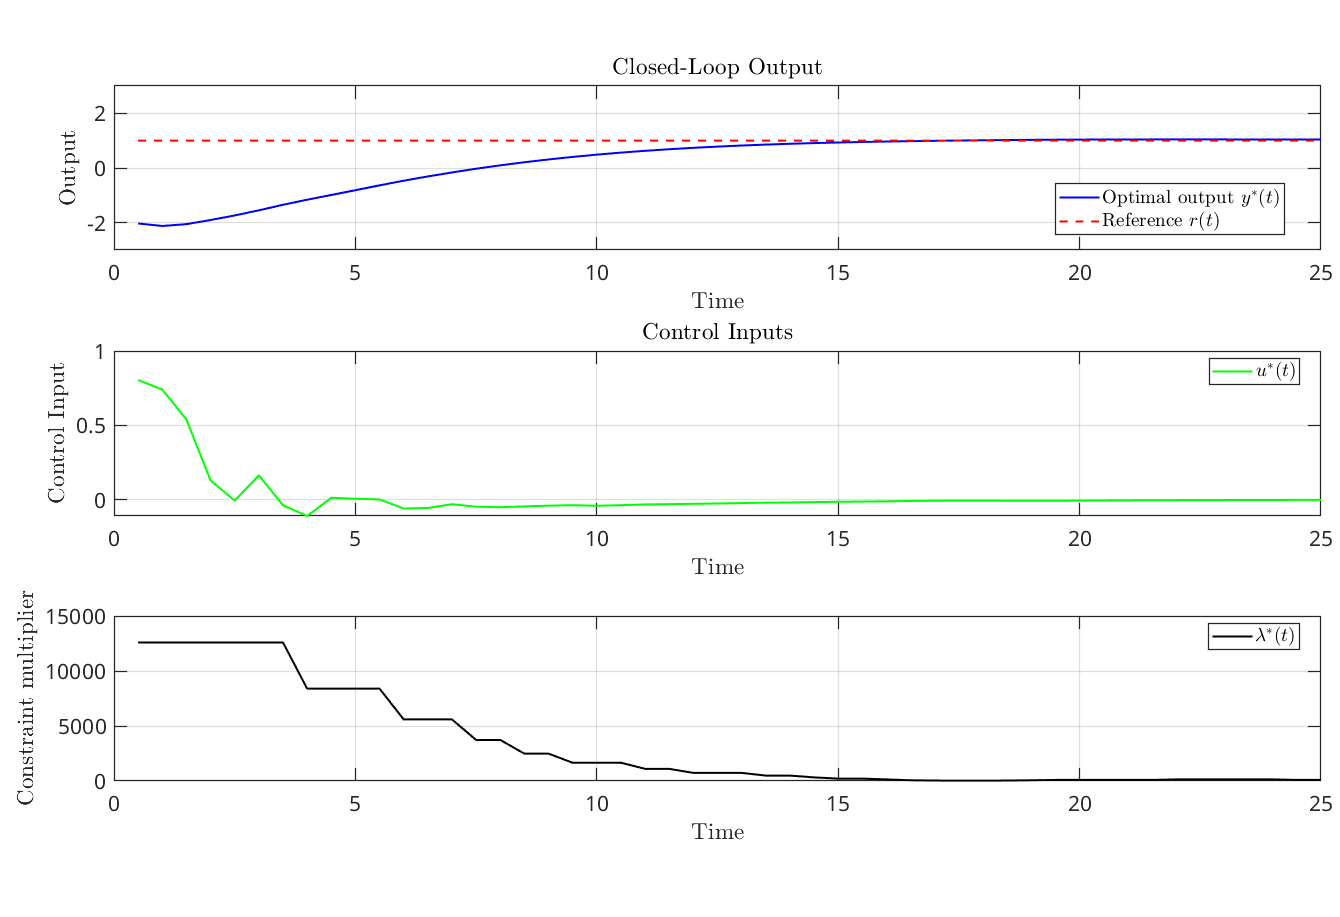
\includegraphics[trim={0cm 1cm 0cm 0cm},clip,width=\textwidth]{figures/closed_loop_noiseless_gamma_5_rho_0p1.png}
    \caption{System simulations for $\sigma = 0$ (no noise).}\label{fig:ddpc_noiseless}
\end{figure}

\textbf{Observations}:
\begin{itemize}
    \item Initially, $\lambda^*$ is large, indicating a significant deviation from the reference trajectory. As the optimization progresses, $Y^*$ aligns better with the true behavior $\hat{Y}$, leading to a decrease in $\lambda^*$.
    \item The optimization algorithm converges within $\sim 30$ iterations per time step on average, demonstrating computational efficiency suitable for real-time applications.
    \item The choice of ball radius $\rho$ significantly impacts the robustness of the control strategy.
\end{itemize}
\begin{figure}[h!]
    \centering
    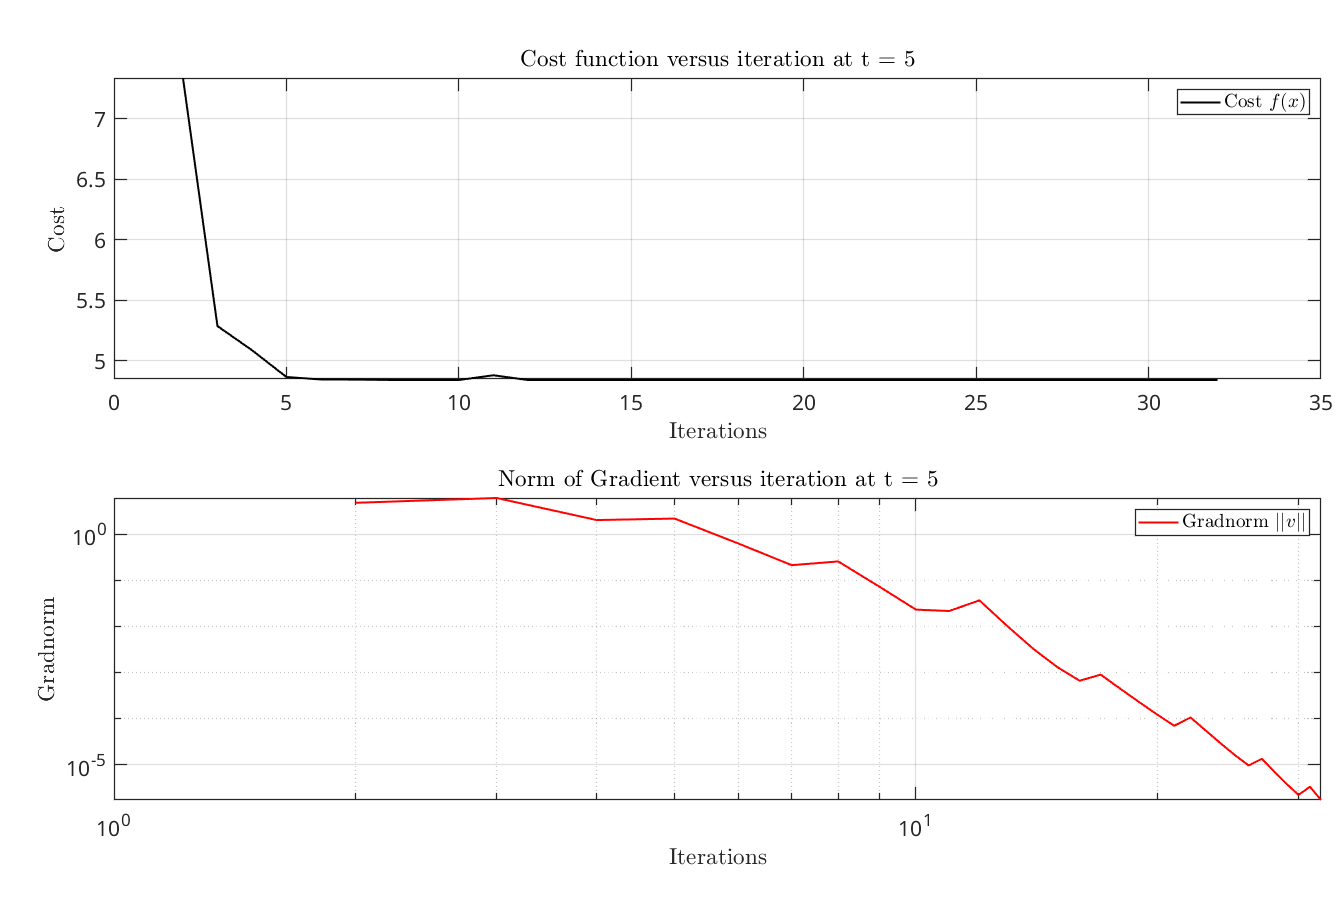
\includegraphics[width=0.9\textwidth]{figures/cost_gradnorm_noiseless_gamma_5_rho_0p1.png}
    \caption{Optimization algorithm convergence at $t=5s$ for $\sigma = 0$ (no noise).}
    \label{fig:conv_noiseless}
\end{figure}

Next, we consider the case with measurement noise ($\sigma = 0.1$). Figures~\ref{fig:ddpc_noisy1} and~\ref{fig:conv_noisy1} illustrate the system simulations and optimization convergence for this scenario. The results show that the robust least-squares approach effectively mitigates the impact of noise, achieving satisfactory tracking performance. The parameters/results for the noisy simulations are summarized in Table~\ref{tab:ddpc_params_double_integrator_noisy1}.
\begin{figure}[h!]
    \centering
    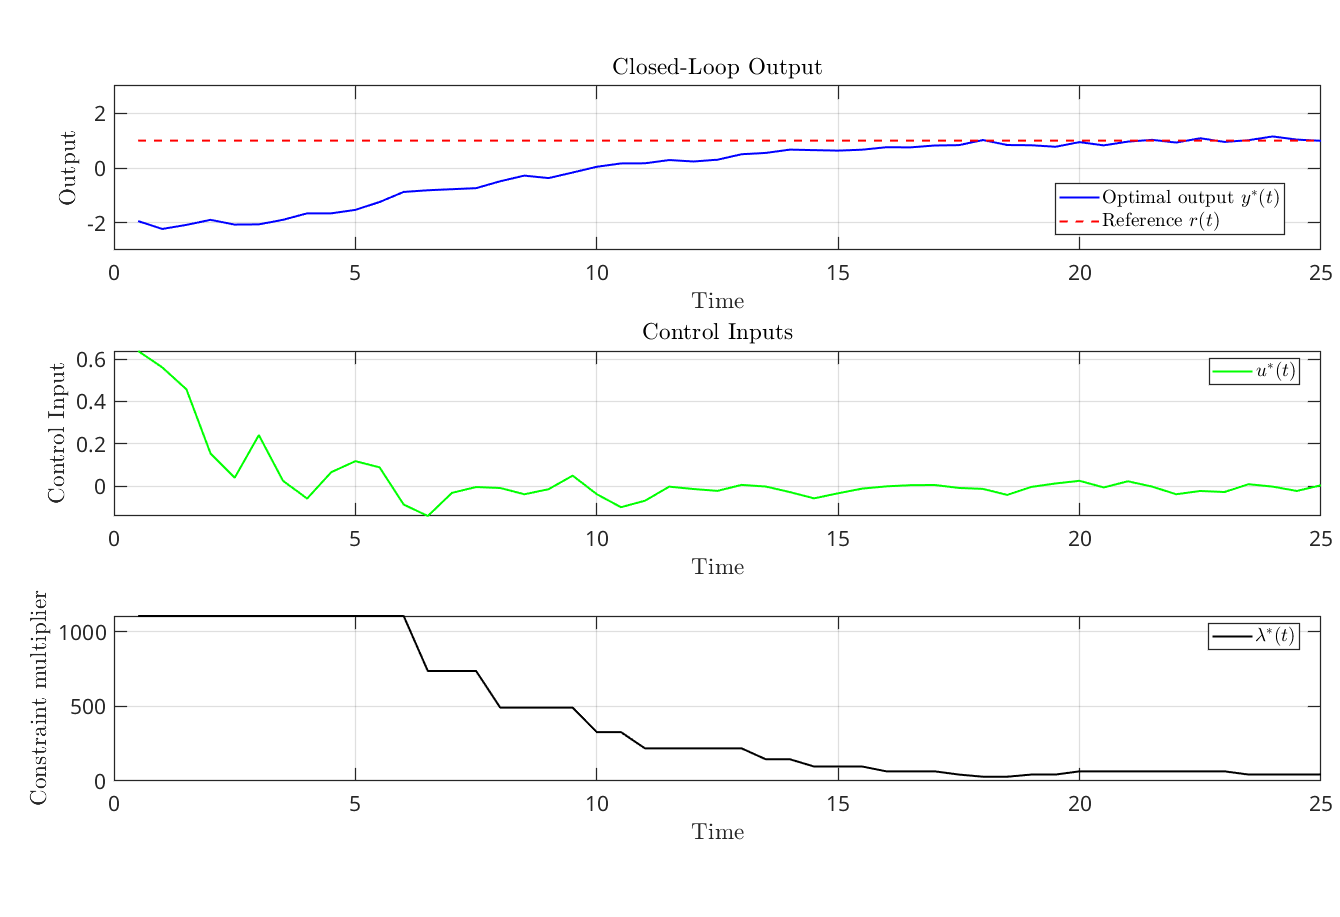
\includegraphics[trim={0cm 1cm 0cm 0cm},clip,width=0.9\textwidth]{figures/closed_loop_snr_0p1_gamma_4_rho_1.png}
    \caption{System simulations for $\sigma = 0.1$ (with noise).}
    \label{fig:ddpc_noisy1}
\end{figure}

\begin{figure}[h]
    \centering
    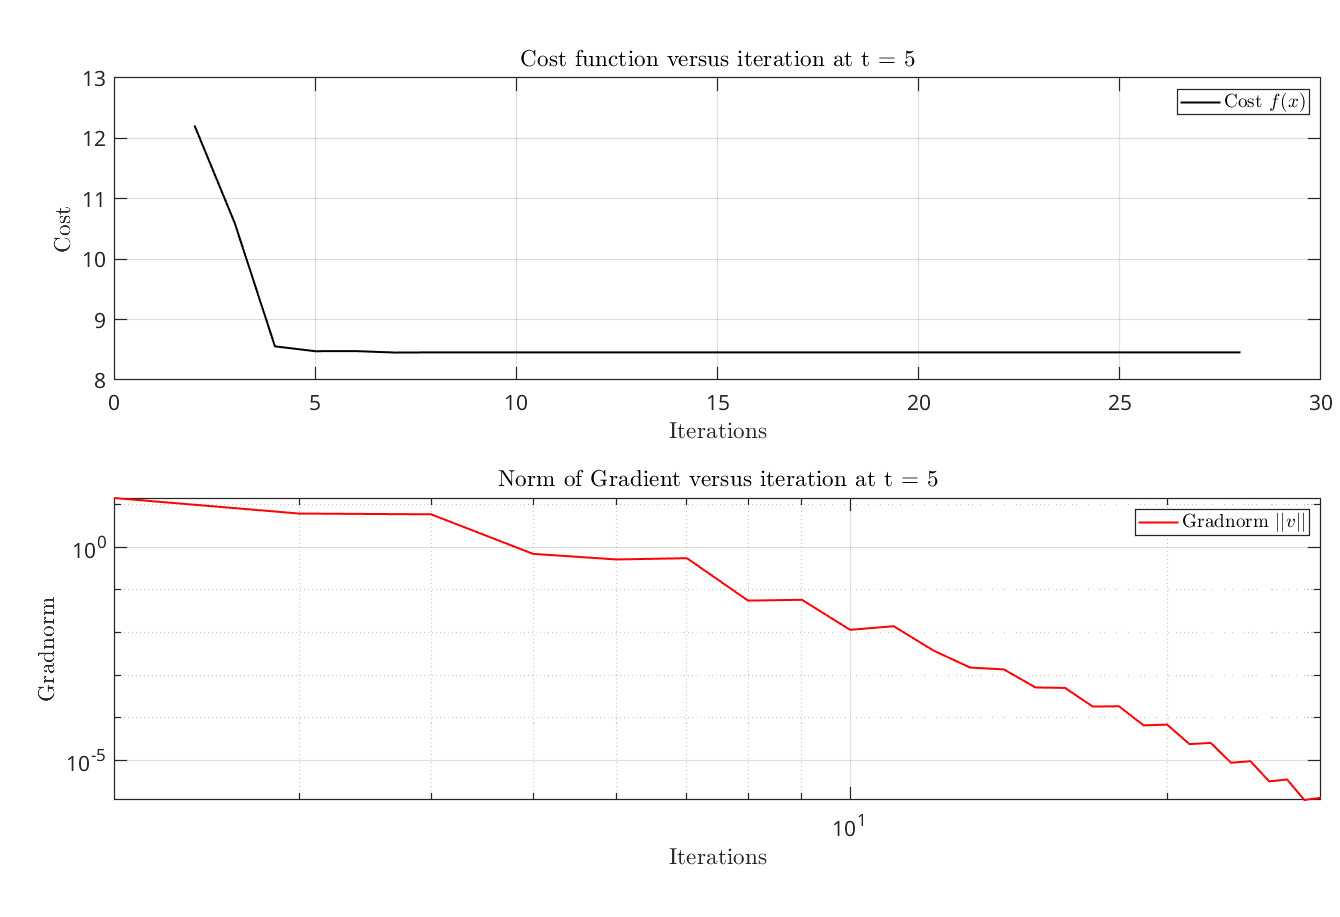
\includegraphics[width=\textwidth]{figures/cost_gradnorm_snr_0p1_gamma_4_rho_1.png}
    \caption{Optimization algorithm convergence at $t=5s$ for $\sigma = 0.1$ (with noise).}
    \label{fig:conv_noisy1}
\end{figure}

\newpage
\begin{table}[h]
    \centering
    \begin{tabular}{l|c}
        \textbf{Parameter} & \textbf{Value} \\
        \hline 
        \hline
        $\rho$ & 1$^\circ$ \\
        $\gamma$ & 4.0 \\
        Total Run-Time & 5.46 s \\
        Tracking Time & 18 s \\
        \hline
    \end{tabular}
    \caption{Simulation parameters/results for $\sigma=0.1$ (with noise)}
    \label{tab:ddpc_params_double_integrator_noisy1}
\end{table}

Now, we further increase the measurement noise to $\sigma = 0.5$. Figures~\ref{fig:ddpc_noisy2} and~\ref{fig:conv_noisy2} illustrate the system simulations and optimization convergence for this higher noise scenario. The robust least-squares approach continues to provide effective tracking performance despite the increased noise level. The parameters/results for the high-noise simulations are summarized in Table~\ref{tab:ddpc_params_double_integrator_noisy2}.

\begin{figure}[h!]
    \centering
    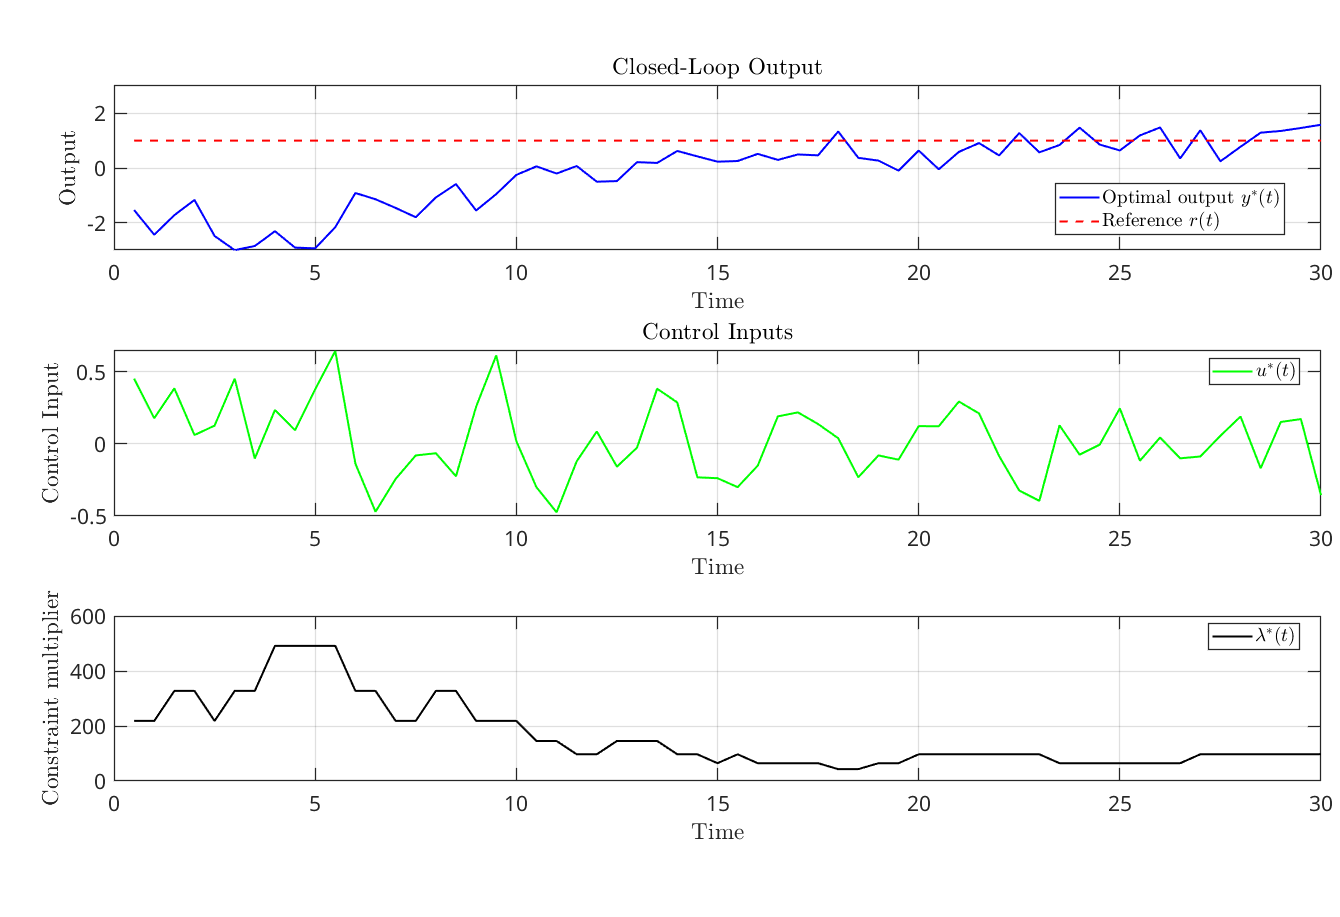
\includegraphics[width=\textwidth]{figures/closed_loop_snr_0p5_gamma_5_rho_3p5.png}
    \caption{System simulations for $\sigma = 0.5$ (with noise).}
    \label{fig:ddpc_noisy2}
\end{figure}
\begin{figure}[h!]
    \centering
    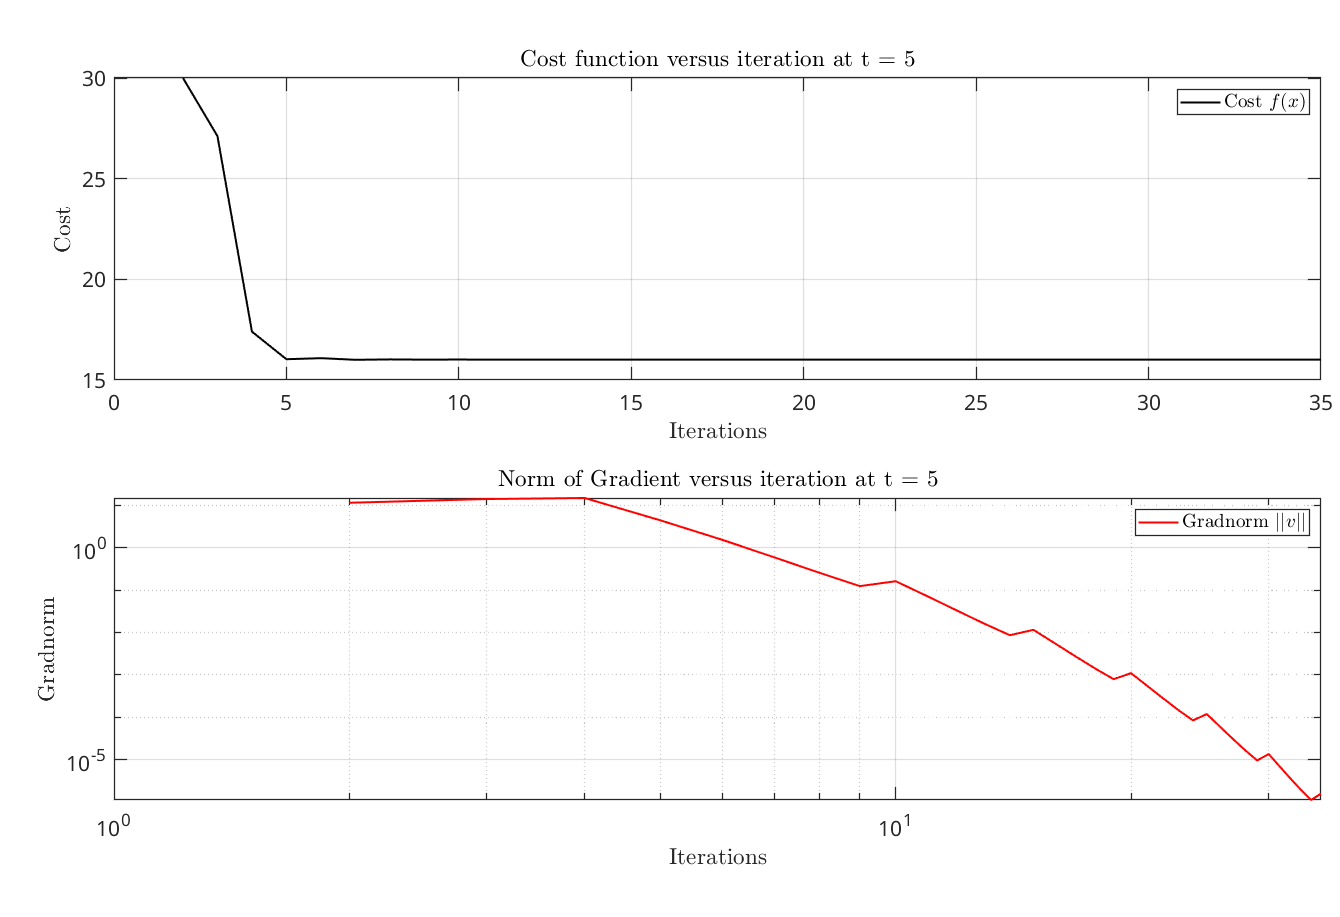
\includegraphics[width=\textwidth]{figures/cost_gradnorm_snr_0p5_gamma_5_rho_3p5.png}
    \caption{Optimization algorithm convergence at $t=5s$ for $\sigma = 0.5$ (with noise).}
    \label{fig:conv_noisy2}
\end{figure} 

\begin{table}[h]
    \centering
    \begin{tabular}{l|c}
        \textbf{Parameter} & \textbf{Value} \\
        \hline 
        \hline
        $\rho$ & 3.5$^\circ$ \\
        $\gamma$ & 5.0 \\
        Total Run-Time & 10.66 s \\
        Tracking Time & 20 s \\
        \hline
    \end{tabular}
    \caption{Simulation parameters/results for $\sigma=0.5$ (with high noise)}
    \label{tab:ddpc_params_double_integrator_noisy2}
\end{table}

\clearpage
\textbf{Observations}:

\begin{itemize}
    \item As the noise level increases, the choice of $\rho$ becomes more critical to maintain robust tracking performance. Remark~\ref{rem:rho} provides insights on how $\rho$ has been estimated in the simulations.
    \item The optimization algorithm remains effective, converging within a reasonable number of iterations even under high noise conditions.
    \item Tuning $\gamma$ helps balance controller performance and algorithm convergence speed. It is yet to be understood how to perform a dynamic update of $\gamma$ during the optimization process for improved results.
\end{itemize}

\begin{remark}\label{rem:rho}
    The ball radius $\rho$ is the quantification of uncertainty in the behavioral estimate $\hat{\Sy}$ (or $\hat{Y}$). As one may expect, increase in measurement noise $\sigma$ should lead to an increase in $\rho$. Although an exact relationship between $\sigma$ and $\rho$ is not yet established, one may estimate $\rho$ as follows.

    Assuming only measurement noise $\eta_k$, denote $\hat{w}_k \in \R^q$ as the noise-free trajectory at time $k$, and $w_k = \hat{w}_k + e_k$ as the actual trajectory, such that
    \[
        e_k = \begin{bmatrix}
            0 \\ \eta_k
        \end{bmatrix} \in \R^q.
    \]
    Let $\hat{Y}$ be the behavioral estimate obtained from system identification (also corrupted by noise). Thus, for online control, the worst-case subspace should contain the worst-case trajectory $w_k$. Note that here, we can assume $\hat{w}_k \in \hat{\Sy}$.  Hence,
    \[
        \rho \approx d_{\infty}(\hat{Y}, Y^*) = \sin(\theta),
    \]
    where $\theta$ is the maximum principle angle between the subspaces $\hat{\Sy}$ and $\Sy_k$ that contains the worst-case trajectory $w_k$. Using basic trigonometry, we thus have
    \[
        \theta = \max_{k} \left\{ \tan^{-1} \left(\dfrac{\lVert P_{\hat{\Sy}}^{\perp} e_k \rVert}{\lVert \hat{w}_k + P_{\hat{\Sy}} e_k \rVert} \right) \right\}.
    \]
\end{remark}

\begin{figure}[h!]
    \centering
    \begin{tikzpicture}[x={(1cm,0cm)}, y={(0.5cm,0.5cm)}, z={(0cm,1cm)}, scale=1.5, >=Stealth]
\fill[blue!20, opacity=0.8] (0,-0.5,0) -- (4,-0.5,0) -- (4,1.5,0) -- (0,1.5,0) -- cycle;
\draw[blue!50, thick] (0,-0.5,0) -- (4,-0.5,0) -- (4,1.5,0) -- (0,1.5,0) -- cycle;
\node at (3.5,0.3,0) {$\hat{\mathcal{S}}$};

\draw[->, thick, blue] (0,0,0) -- (2.8,0.7,0) node[midway, below right ] {$\hat{w}_k$};

\fill[red!30, opacity=0.8, rotate=20] (0,-0.5,0) -- (4.5,-0.5,0) -- (4.5,1.5,0) -- (0,1.5,0) -- cycle;
\draw[red!50, thick, rotate=20] (0,-0.5,0) -- (4.5,-0.5,0) -- (4.5,1.5,0) -- (0,1.5,0) -- cycle;

\draw[->, thick, red] (0,0,0) -- (3.5,1,1) node[midway, above left] {$w_k$};
\node at (3.7,1,1.5) {$\mathcal{S}_k$};

\draw[->,thick,purple] (2.8,0.7,0) -- (3.5,1,1) node[midway, right] {$e_k$};
\draw[dashed, purple] (3.5,1,0) -- (3.5,1,1) node[midway, right] {$P_{\hat{\mathcal{S}}}^{\perp} e_k$};
\draw[thick, purple] (3.4,1,0.1) -- (3.5,1,0.15);
\draw[thick, purple] (3.4, 1,0.11) -- (3.4,1.01,-0.05);

\node at (0.9,0,0.23) {$\theta$};
\path[clip] (2,0.5,0) -- (0,0,0) -- (2,1,0.4) -- cycle;
\node[circle,draw=black,minimum size=60pt,thick] at (0,0,0) (circ) {};

\end{tikzpicture}
\caption{Estimation of ball radius $\rho$ based on trajectory deviation $e_k$.}
\end{figure}